\documentclass[sigconf,anonymous,review]{acmart}

% ACM FAccT submission (anonymous review build). Compiles with the ACM `acmart`
% class (built in on Overleaf; otherwise `tlmgr install acmart`).

\usepackage{amsmath,amssymb}
\usepackage{booktabs}
\usepackage{graphicx}

\settopmatter{printacmref=false}
\renewcommand\footnotetextcopyrightpermission[1]{}
\pagestyle{plain}

\newtheorem{theorem}{Theorem}
\newtheorem{proposition}{Proposition}

\begin{document}

\title{The Individuation Gap: an Accountability Boundary for Individual
Inference from Predicted Brains}

\author{Anonymous Author(s)}
\affiliation{%
  \institution{Submission under double-blind review}
  \country{}
}

\begin{abstract}
A growing market claims to infer an individual's mental state or behaviour from brain and body signals, and
increasingly from a \emph{predicted} brain: an encoder maps media or context to cortical activity, which is
then read as if it had been measured. These claims carry accountability stakes, because they assert
knowledge about specific people and are sold to advertisers, employers, and clinicians. We give a precise
and verifiable boundary on what such systems can deliver. Forecasting value separates into a population part
and an individual part. The population part improves with aggregation, which we prove; the individual part
depends on between-subject variance that a zero-shot encoder does not carry, so it is zero without
per-subject enrollment. On three real datasets the consequence is stark: non-invasive readouts recover
\emph{who} a person is (in-scanner fingerprinting at 100\%; a behavioural fingerprint at 14 times chance)
but not \emph{what} they will do (the individual neural-to-behaviour link abstains under a calibrated test).
A Bayes-optimal forecaster inherits the limit, and combining modalities does not remove it. The findings
expose an information-asymmetry problem: a vendor can verify or re-identify a person far more readily than it
can read their mind, yet the mind-reading claim is the one marketed. We translate the boundary into a
refusal-first read-out and a disclosure standard that separates identity from content, and we connect both
to emerging biometric and AI regulation.
\end{abstract}

\keywords{neurotechnology, individual inference, accountability, transparency, information asymmetry,
biometric categorization, auditing, calibration}

\maketitle

\section{Introduction}
Algorithmic systems that infer things about people are the central concern of fairness, accountability, and
transparency. A fast-growing class of such systems infers mental content: affective-computing products,
brand-intelligence platforms, and personalized neuro-mental-health tools that claim to read a person's
emotion, attention, or likely choice from brain or body signals. Many do so from a \emph{predicted} brain,
where an encoder maps a stimulus to cortical activity that is then labelled with construct names and sold as
a measurement \citep{poldrack2006,hutzler2013}.

The accountability question is whether these individual claims can be true. If they cannot, the asymmetry is
severe: the vendor asserts private knowledge about a specific person, the person cannot contest it, and the
claim resists audit because it is framed as a scientific measurement. We give a boundary that makes the
claim auditable. Forecasting value from a predicted brain separates into a population part and an individual
part, and the two behave differently. The population part is tractable and grows with aggregation; the
individual part is bounded by the encoder and, for a person the encoder never saw, is empty. We call this the
individuation gap, prove it, confirm it on synthetic data, and show three real datasets fall where it
predicts (Figure~\ref{fig:overview}). We then turn the boundary into governance: a read-out that withholds
unearned individual claims, and a disclosure that keeps identity recognition, which does work, separate from
mental-content reading, which does not.

\begin{figure}[t]
\centering
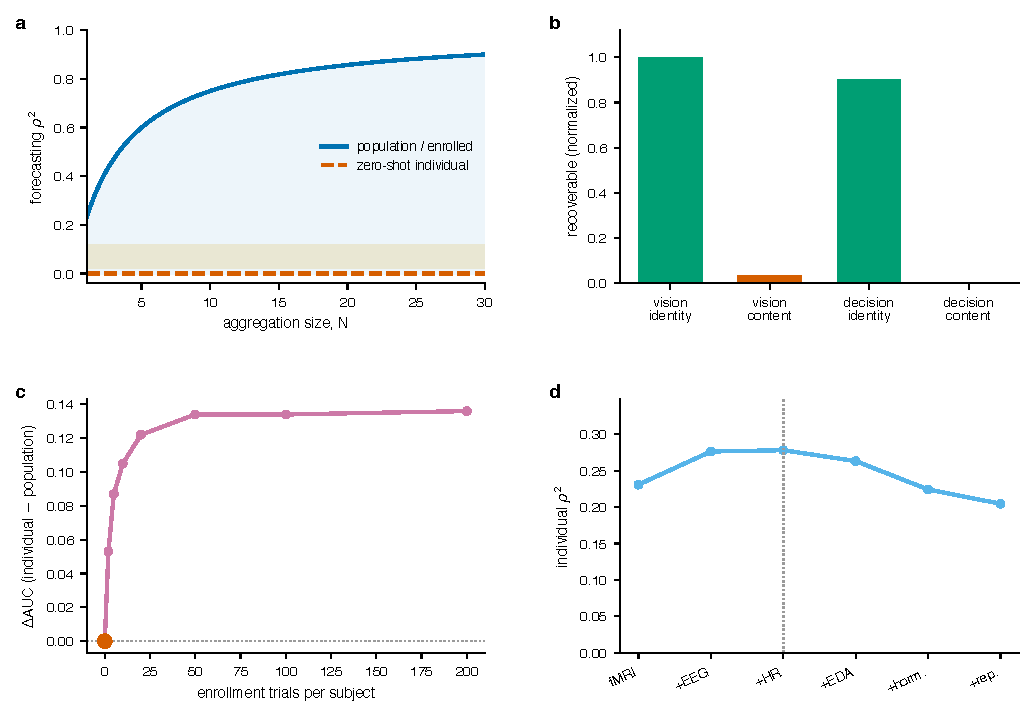
\includegraphics[width=\columnwidth]{../figures/fig0_overview.pdf}
\caption{The individuation gap. (a) The population term rises with aggregation while the zero-shot individual
term is zero, below the small measured individual-difference ceiling \citep{marek2022}. (b) On real data,
identity is recoverable while individual behavioural content is not. (c) A Bayes-optimal forecaster gains no
individual value at zero-shot. (d) Fusion is non-monotone: low-reliability modalities lower individual
$\rho^2$.}
\label{fig:overview}
\end{figure}

\section{The individuation gap}
Let an outcome be $Y=S+\varepsilon$ with idiosyncratic-noise variance $v>0$, and let the predictor resolve an
identifiable between-unit signal variance $a\ge 0$. The best-case squared correlation is
\begin{equation}
\rho^2(a,v)=\frac{a}{a+v}.
\label{eq:rho}
\end{equation}
Aggregating over $N$ units replaces $v$ with $v/N$; a zero-shot encoder has $a=0$.

\begin{theorem}[Population]\label{thm:agg} For $a,v>0$, $N>1$: $\rho^2(a,v)<\rho^2(a,v/N)$.\end{theorem}
\begin{theorem}[Zero-shot individual]\label{thm:zero} For all $v,N$: $\rho^2(0,v/N)=0$.\end{theorem}
\begin{theorem}[The gap]\label{thm:gap} For $a,v>0$, $N>0$: $\rho^2(0,v/N)<\rho^2(a,v/N)$.\end{theorem}

Theorem~\ref{thm:zero} is the accountability-relevant one: a predictor with no between-unit variance has zero
best-case correlation with the individual component, at any noise level and any sample size, because the
quantity it would estimate is absent from the input. The three statements are machine-checked in Lean~4 with
Mathlib, so the boundary rests on a proof.

\section{Identity is recoverable, behaviour is not}
Across three real datasets, enrollment buys identity rather than behaviour (Table~\ref{tab:real}).
Subject-specific image-to-fMRI encoders ($N{=}8$) identify the subject in all 25 regions at 100\% (chance one
in eight), while the behaviourally relevant geometry is small ($0.005$ to $0.066$) and capped by the stimulus
representation \citep{allen2022,chang2019}. A decision phenotype from 107 people and about 27{,}000 choices
identifies individuals at 14 times chance ($p=5\times10^{-4}$) and predicts held-out choices at AUC $0.965$
with conformal coverage $1.00$, yet the direct individual neural-to-behaviour link abstains under a calibrated
test \citep{botviniknezer2019,tom2007}. The who question is answerable; the what question is not.

\begin{table}[t]
\centering\small
\caption{Identity recovers in every setting; individual behavioural content does not.}
\label{tab:real}
\begin{tabular}{@{}p{3.1cm}p{2.0cm}p{2.0cm}@{}}
\toprule
Setting & Identity (who) & Content (what) \\
\midrule
Vision encoding ($N{=}8$) & 25/25 at 100\% & $0.005$--$0.066$ \\
Value decision ($N{=}107$) & 14$\times$ chance & abstains \\
Value decision, aggregate & AUC $0.965$ & baseline dominates \\
\bottomrule
\end{tabular}
\end{table}

\section{The limit is not an engineering gap}
A Bayes-optimal forecaster inherits the limit: with a predictor constant across subjects, the posterior over
an individual's outcome equals the population prior, and mutual information with the individual outcome is
zero (Proposition~\ref{prop:bayes}). In simulation, incremental individual AUC over the population model is
$0.000$ at zero-shot and rises only to about $0.14$ after 200 per-subject trials. Combining modalities does
not help in general: each added signal contributes variance as well as signal, so individual $\rho^2$ is
non-monotone in the number of modalities (Proposition~\ref{prop:fusion}).

\begin{proposition}[Posterior collapse]\label{prop:bayes}
A predictor constant across subjects is independent of the individual outcome given the population; the
Bayes-optimal individual forecast equals the population forecast.
\end{proposition}
\begin{proposition}[Fusion is not monotone]\label{prop:fusion}
Adding a modality with per-modality signal $a_m$ and added noise $\delta_m$ raises individual $\rho^2$ only if
$a_m/\delta_m$ exceeds the current signal-to-noise ratio; low-reliability modalities lower it.
\end{proposition}

These agree with the measurement literature: brain-wide individual effects are small ($r\approx0.14$ to
$0.34$) and need thousands of subjects \citep{marek2022,kang2024}; task-fMRI individual reliability is poor
(mean ICC $0.397$) \citep{elliott2020,kragel2021}; and individual precision mapping takes hours of data per
person \citep{gordon2017,du2025}.

\section{Accountability implications}
\paragraph{Information asymmetry.} The gap formalizes a specific asymmetry. A vendor holding a predicted-brain
readout can verify or re-identify a person far more readily than it can read that person's mental content, yet
the mental-content claim is the one marketed and the one that most affects the person. Buyers, regulators, and
the people being scored cannot easily tell the two apart, because both are reported as neural measurements.

\paragraph{A refusal-first read-out and a disclosure standard.} We translate the boundary into a read-out
that returns a construct score only when the construct has a meta-analytic localizer, the predicted index
beats a stimulus-only baseline, and the score carries a conformal interval \citep{vovk2005}. Identity and
content are reported on separate, separately-governed channels, so a system may verify who a person is
without asserting what they think. This gives auditors a concrete test and vendors a standard that reports a
value only when it is supported.

\paragraph{Regulatory connection.} The identity result, which does work, is a biometric capability and should
carry the safeguards that regimes such as the EU AI Act attach to biometric identification and emotion
inference. The content result, which does not work non-invasively, indicates that individual
emotion-recognition and intent-prediction claims from predicted brains are, at present, unsupportable and
should be treated as such in procurement and disclosure.

\section{Discussion and limitations}
The synthetic and Bayesian results check the method and the probability claim, not any specific product. The
three real-data results were produced under separate analyses, so they are convergent evidence rather than
one preregistered study, and the decision-fMRI link abstains at the edge of power. The model in
Equation~\ref{eq:rho} is a best-case abstraction; richer encoders change the constants but not the sign of the
gap, since $a=0$ for any zero-shot predictor. The invasive exception is real: intracortical interfaces and
optogenetics reach the individual by recording or perturbing that individual's own circuitry
\citep{willett2023,card2025,silva2024,zhao2011,bernalcasas2017}, which is exactly the signal a non-invasive
zero-shot readout lacks, and which carries its own, stricter governance questions.

\bibliographystyle{ACM-Reference-Format}
\begin{thebibliography}{00}
\bibitem{allen2022} E.~J. Allen et al. 2022. A massive 7T fMRI dataset. \emph{Nature Neuroscience} 25 (2022), 116--126.
\bibitem{bernalcasas2017} D. Bernal-Casas et al. 2017. Dynamic causal modeling for optogenetic fMRI. \emph{Neuron} 93, 3 (2017), 522--532.
\bibitem{botviniknezer2019} R. Botvinik-Nezer et al. 2019. A large-scale fMRI dataset for value-based decision making. \emph{Scientific Data} 6 (2019), 106.
\bibitem{card2025} N.~S. Card et al. 2026. Long-term independent use of an intracortical BCI. \emph{Nature Medicine} 32, 7 (2026), 2504--2510.
\bibitem{chang2019} N. Chang et al. 2019. BOLD5000. \emph{Scientific Data} 6 (2019), 49.
\bibitem{dmochowski2014} J.~P. Dmochowski et al. 2014. Audience preferences predicted by temporal reliability of neural processing. \emph{Nature Communications} 5 (2014), 5567.
\bibitem{du2025} J.-N. Du et al. 2025. Within-individual precision mapping using task data. \emph{Neuron} (2025).
\bibitem{elliott2020} M.~L. Elliott et al. 2020. Test-retest reliability of task-fMRI measures. \emph{Psychological Science} 31, 7 (2020), 792--806.
\bibitem{gordon2017} E.~M. Gordon et al. 2017. Precision functional mapping of individual human brains. \emph{Neuron} 95, 4 (2017), 791--807.
\bibitem{hutzler2013} F. Hutzler. 2013. Reverse inference is not a fallacy per se. \emph{NeuroImage} 84 (2013), 1061--1069.
\bibitem{kang2024} K. Kang et al. 2024. Study design features increase replicability in BWAS. \emph{Nature} 636, 8043 (2024), 719--727.
\bibitem{kragel2021} P.~A. Kragel et al. 2021. Functional MRI can be highly reliable. \emph{Psychological Science} 32, 4 (2021), 622--626.
\bibitem{marek2022} S. Marek et al. 2022. Reproducible brain-wide association studies require thousands of individuals. \emph{Nature} 603 (2022), 654--660.
\bibitem{poldrack2006} R.~A. Poldrack. 2006. Can cognitive processes be inferred from neuroimaging data? \emph{Trends in Cognitive Sciences} 10, 2 (2006), 59--63.
\bibitem{silva2024} A.~B. Silva et al. 2024. The speech neuroprosthesis. \emph{Nature Reviews Neuroscience} 25, 7 (2024), 473--492.
\bibitem{tom2007} S.~M. Tom et al. 2007. The neural basis of loss aversion. \emph{Science} 315, 5811 (2007), 515--518.
\bibitem{vovk2005} V. Vovk, A. Gammerman, and G. Shafer. 2005. \emph{Algorithmic Learning in a Random World}. Springer.
\bibitem{willett2023} F.~R. Willett et al. 2023. A high-performance speech neuroprosthesis. \emph{Nature} 620 (2023), 1031--1036.
\bibitem{yao2024} X. Yao et al. 2024. Using neural data to forecast aggregate consumer behavior. \emph{Journal of Consumer Behaviour} (2024).
\bibitem{zhao2011} S. Zhao et al. 2011. Cell type-specific channelrhodopsin-2 transgenic mice. \emph{Nature Methods} 8, 9 (2011), 745--752.
\end{thebibliography}

\end{document}
